%
% CHAPTER 7.- Interesting Questions
%

\chapterimage{thinker.pdf}

\chapter{Interesting Questions}
\label{chap:Interesting-Research-Questions}

\begin{quote}
\begin{flushright}
\emph{It is not the answer that enlightens,\\
but the question. \\}
Eugène Ionesco
\end{flushright}
\end{quote}
\bigskip

In this chapter, we introduce a set of metrics for classifying research topics according to their potential to generate interesting problems, along with a methodology for the assisted discovery of new research questions. The objective is to propose new directions, novel research ideas, that contribute to reducing nescience, that is, to diminishing the extent of the scientific unknown. The proposed methodology supports both the identification of new applications for existing tools to address open problems (the known unknown\index{Known unknown}) and the discovery of entirely new and previously unexplored research directions (the unknown unknown\index{Unknown unknown}). While the methodology is applicable to both intradisciplinary and interdisciplinary topics, the most impactful results typically arise in the latter case. In Chapter \ref{chap:computational-creativity}, we demonstrate the methodology in practice and propose several new questions and research topics.

We have already examined three dimensions for classifying research topics: miscoding (Chapter \ref{chap:Miscoding}), inaccuracy (Chapter \ref{chap:Error}), and surfeit (Chapter \ref{chap:Redundancy}). These metrics allow us to quantitatively assess our level of understanding of a topic, a concept we refer to as nescience. In this section, we introduce two additional metrics for characterizing topics: relevance (Section \ref{sec:relevance}) and applicability (Section \ref{sec:applicability}). Relevance measures the impact a topic has on people's lives and complements the existing metrics of nescience. Applicability quantifies how frequently a topic has been applied in other domains and helps identify new uses for existing technologies.

What is proposed in this chapter is an algebraic approach to the assisted discovery of potentially interesting research questions, grounded in the theory of nescience. The objective of this methodology is twofold. On the one hand, it aims to support researchers in their day-to-day work. The methodology can be used to uncover novel tools that may be applied to a given problem, or to identify new problems where existing tools could be effectively used. In its more advanced form, the methodology facilitates the exploration of the unknown unknown, that is, research areas that have not yet been conceptualized, described, or even imagined.

On the other hand, because the methodology is based on well-defined mathematical principles, it lends itself to automation. This opens the door for artificial intelligence systems to move beyond their current limitations, namely, their inability to autonomously generate truly novel research directions. By formalizing the process of question discovery, the methodology enables AI to propose interesting and previously unexplored research questions, and even to discover entirely new topics of scientific inquiry.

%
% Relevance
%

\section{Relevance}
\label{sec:relevance}

In this chapter, we propose additional metrics to complement nescience in the task of evaluating the interest of research topics. These metrics will be useful not only for classifying individual topics, but also for developing a methodology for discovering potential solutions to open problems (Section \ref{sec:intro_interesting_questions}), as well as for identifying entirely new research topics (Section \ref{sec:New_Research_Topics}).

One of these new metrics is \emph{relevance}. Relevance quantifies the impact that a research topic has on people's lives. Intuitively, the greater the relevance of a topic, the higher its potential as a source of interesting problems, since it concerns issues that affect many individuals directly.

Before we can measure the relevance of a topic, that is, its impact on people's lives, we must introduce the concept of a \emph{relevance graph}. The relevance graph (see Figure \ref{fig:Relevance-Graph}) captures the relationship between people and the research topics that affect them.

\begin{definition}\index{Relevance Graph}
\label{def:relevance-graph}
We define the \emph{relevance graph}\index{Relevance graph}, denoted by $\mathbf{RG}$, as the bipartite graph $\mathbf{RG} = (\mathcal{T}, \mathcal{P}, E)$, where $\mathcal{T}$ is the set of topics, $\mathcal{P}$ is the set of people, and $E\subseteq\left\{ \left(i,j\right):i\in \mathcal{T},j\in \mathcal{P} \right\}$ is the set of edges between topics and people. An edge $(i, j)$ belong to $E$ if, and only if, person $j$ is affected by topic $i$.
\end{definition}

When we refer to the set of people $\mathcal{P}$, we mean all individuals in the world. A connection between a topic and a person indicates that the person is affected by the topic, not that they are necessarily interested in it. For example, someone researching a cure for diabetes would not be connected to the research topic "diabetes," but someone who actually suffers from the disease would be.

The higher the relevance of a topic, the greater its potential as a source of interesting problems to solve. In this sense, the research topic "how to cure diabetes" is more relevant than "how far dog fleas can jump," because more people are affected by the former than by the latter.

The precise meaning of "\emph{being affected by}" is inherently abstract and must be approximated in practice. For instance, one could argue that the spouse of a person with diabetes is also affected by the disease in some way. In Section \ref{sec:relevance_in_practice}, we will explore how this concept can be operationalized in the context of scientific research topics.

% \begin{figure}[h]
% \centering\includegraphics[scale=0.7]{bipartite_graph}
% \caption{\label{fig:Relevance-Graph}Relevance Graph}
% \end{figure}

\begin{figure}[t]
\centering
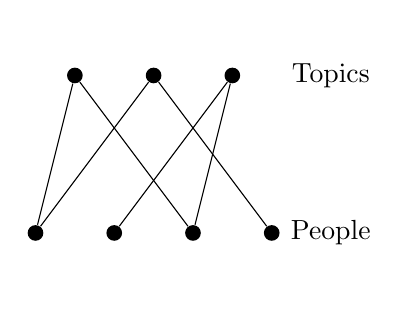
\begin{tikzpicture}[scale=1, every node/.style={circle, fill=black, inner sep=2pt}]

% Nodes: Topics (top row)
\node (t1) at (0.5,2) {};
\node (t2) at (1.5,2) {};
\node (t3) at (2.5,2) {};

% Nodes: People (bottom row)
\node (p1) at (0,0) {};
\node (p2) at (1,0) {};
\node (p3) at (2,0) {};
\node (p4) at (3,0) {};

% Edges
\draw (t1) -- (p1);
\draw (t1) -- (p3);
\draw (t2) -- (p1);
\draw (t2) -- (p4);
\draw (t3) -- (p2);
\draw (t3) -- (p3);

% Labels
\node[draw=none, fill=none] at (3.75,2) {Topics};
\node[draw=none, fill=none] at (3.75,0) {People};

\end{tikzpicture}
\caption{\label{fig:Relevance-Graph}Relevance Graph}
\end{figure}

Optionally, we can assign a weight $w_{ij} \in [0,1]$ to the edges of the graph to indicate the degree to which a person $j$ is affected by a topic $i$. A weight of $1$ could represent a life-or-death dependence, while a weight of $0$ would mean that the person is not affected at all. Figure \ref{fig:Relevance-Graph} shows an example of a relevance graph.

The relevance of a topic measures the extent to which it affects people. This can be assessed either by counting the number of affected individuals or by taking into account the magnitude of the effect.

\begin{definition}\index{Relevance}
\label{def:relevance}
Let $t \in \mathcal{T}$ be a topic, $\mathcal{P}_t \subseteq \mathcal{P}$ the set of people connected to $t$ in the relevance graph, and $w_{tp} \in [0,1]$ the weight of the edge between $t$ and $p \in \mathcal{P}_t$. We define the \emph{relevance} of $t$ as
\[
R(t) = \sum_{p : (t,p) \in E} w_{tp},
\]
\end{definition}

The unweighted relevance $R(t)$ (with $w_{tp} = 1$) counts the number of people affected by the topic, while the weighted relevance $R(t)$ reflects both the number of people and the severity of the effect. A higher relevance value indicates greater potential for generating important and impactful questions.

In practice it is useful to normalize the relevance of a topic so that the least relevant topic has a value of $0$, the most relevant has a value of $1$, and all others lie proportionally in between.

\begin{definition}\index{Normalized relevance}
\label{def:minmax_normalized_relevance}
Let $t \in \mathcal{T}$ be a topic. We define the \emph{min-max normalized relevance} of $t$ as
\[
\bar{R}(t) = \frac{R(t) - \min_{t' \in \mathcal{T}} R(t')}{\max_{t' \in \mathcal{T}} R(t') - \min_{t' \in \mathcal{T}} R(t')}
\]
\end{definition}

This transformation ensures that $\bar{R}(t) \in [0,1]$, with $0$ assigned to the least relevant topic and $1$ to the most relevant. In the degenerate case where all topics have the same relevance, all normalized values are set to $0$.

We could also compute the weighted degree of a person $p$, denoted $R(p)$, defined as the sum of the weights of the edges that link $p$ to topics in the relevance graph. This quantity measures the overall impact of all topics on a particular person. However, this measure is not used in the theory of nescience.

The relation between the weighted relevance of topics and the weighted degrees of people is given by the weighted degree sum formula:
\[
\sum_{t \in \mathcal{T}} R(t) \;=\; \sum_{p \in \mathcal{P}} R(p) \;=\; \sum_{(t,p) \in E} w_{tp}.
\]
In the unweighted case ($w_{tp} = 1$ for all edges), this formula reduces to the standard degree sum formula
\[
\sum_{t \in \mathcal{T}} \deg(t) \;=\; \sum_{p \in \mathcal{P}} \deg(p) \;=\; d(E).
\]

The next proposition shows that, in the weighted case, adding more topics to a research project can only increase its overall relevance. Of course, a research project dealing with "life, the universe, and everything" would be highly relevant, but also highly impractical. How to properly combine research topics will be described in Section \ref{sec:New_Research_Topics}.

\begin{proposition}
Let $S \subseteq \mathcal{T}$ be a finite set of topics and let $t' \in \mathcal{T} \setminus S$ be an additional topic. Then
\[
R(S \cup \{t'\}) \;\geq\; R(S),
\]
where the total weighted relevance of a set of topics $S$ is defined as
\[
R(S) = \sum_{\substack{t \in S \\ p \in \mathcal{P} \\ (t,p) \in E}} w_{tp}.
\]
\end{proposition}
\begin{proof}
We can write
\[
R(S \cup \{t'\}) = \sum_{\substack{t \in S \cup \{t'\} \\ p \in \mathcal{P} \\ (t,p) \in E}} w_{tp}
= R(S) + \sum_{\substack{p \in \mathcal{P} \\ (t',p) \in E}} w_{t'p}.
\]
Since all weights $w_{tp}$ are non-negative,
\[
\sum_{\substack{p \in \mathcal{P} \\ (t',p) \in E}} w_{t'p} \geq 0,
\]
which implies $R(S \cup \{t'\}) \geq R(S)$.
\end{proof}

This property shows that weighted relevance is monotone with respect to topic inclusion: if you enlarge the set of topics under consideration, the total weighted relevance can never decrease. In other words, adding topics can only maintain or increase the number (or severity) of connections to people in the relevance graph.

%
% Applicability
%

\section{Applicability}
\label{sec:applicability}

In this section, we introduce a new metric, applicability, which measures the potential of a research topic to serve as a tool for understanding or solving problems in other topics. The intuition is that some topics act as powerful enablers: mastering them allows progress to be made in many other areas.

From a formal standpoint, we say that a topic $t_j$ can be applied to a topic $t_i$ if the conditional nescience of $t_i$ given $t_j$ is smaller than the unconditional nescience of $t_i$ (see Section \ref{sec:conditional_nescience}).

Before defining applicability formally, we introduce the applicability graph, which encodes which topics have been successfully applied to others. This is a directed graph whose nodes are research topics, and where an arc from $t_j$ to $t_i$ indicates that $t_j$ has been successfully applied to explain or solve $t_i$.

\begin{definition}\index{Applicability graph}
\label{def:applicability-graph}
We define the \emph{applicability graph}, denoted by $AG$, as the directed graph $AG = (\mathcal{T}, E)$, where $\mathcal{T}$ is the set of research topics, and $E \subseteq \{ (i,j) : i,j \in \mathcal{T} \}$ is the set of arcs. An arc $(i,j)$ belongs to $E$ if $N(t_i \mid t_j) < N(t_i)$, that is, knowing $t_j$ reduces the nescience of $t_i$. The weight of the arc $(i,j)$ is defined as $w_{ij} = N(t_i) - N(t_i \mid t_j)$, representing the reduction in nescience obtained by applying $t_j$ to $t_i$.
\end{definition}

\begin{figure}[t]
\centering
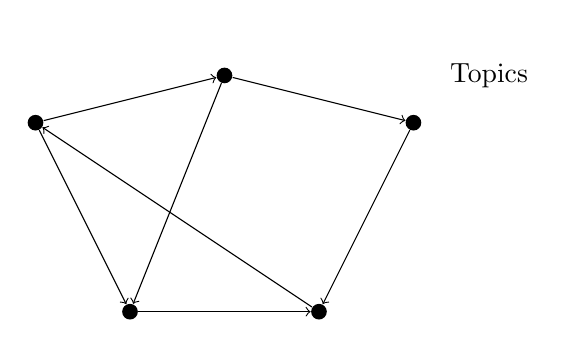
\begin{tikzpicture}[scale=1.2, every node/.style={circle, fill=black, inner sep=2pt}]

% Nodes (topics)
\node (t1) at (0,2) {};
\node (t2) at (2,2.5) {};
\node (t3) at (4,2) {};
\node (t4) at (1,0) {};
\node (t5) at (3,0) {};

% Directed edges
\draw[->] (t1) -- (t4);
\draw[->] (t1) -- (t2);
\draw[->] (t2) -- (t3);
\draw[->] (t2) -- (t4);
\draw[->] (t3) -- (t5);
\draw[->] (t4) -- (t5);
\draw[->] (t5) -- (t1);

% Labels
\node[draw=none, fill=none] at (4.8,2.5) {Topics};

\end{tikzpicture}
\caption{\label{fig:ApplicabilityGraph}Example of an applicability graph.}
\end{figure}

The applicability of a topic measures the total reduction in nescience it has produced when applied to other topics.

\begin{definition}\index{Applicability}
\label{def:applicability}
Given the applicability graph $AG = (\mathcal{T}, E)$, the \emph{applicability} of a topic $t_i \in \mathcal{T}$, denoted $A(t_i)$, is defined as
\[
A(t_i) = \sum_{(i,j) \in E} w_{ij},
\]
where the sum is over all arcs leaving $t_i$.
\end{definition}

A topic with high applicability is a versatile tool, capable of contributing to the understanding of many other topics. Intuitively, if a tool has been successfully applied multiple times in the past, it is more likely to be useful for solving new problems in the future.

As with relevance, applicability is monotone with respect to topic inclusion: combining topics can only increase their total applicability.

\begin{proposition}
\label{prop:nondecreasing_applicability}
Let $S \subseteq \mathcal{T}$ be a finite set of topics and $t' \in \mathcal{T} \setminus S$ an additional topic. Then
\[
A(S \cup \{t'\}) \geq A(S),
\]
where
\[
A(S) = \sum_{\substack{t \in S \\ (t,j) \in E}} w_{tj}.
\]
\end{proposition}
\begin{proof}
We can write
\[
A(S \cup \{t'\}) = A(S) + \sum_{(t',j) \in E} w_{t'j}.
\]
Since all weights $w_{ij}$ are non-negative,
\[
\sum_{(t',j) \in E} w_{t'j} \geq 0,
\]
which implies $A(S \cup \{t'\}) \geq A(S)$.
\end{proof}

This property ensures that adding more tools to a research effort can only maintain or increase its applicability.

To compare applicability values across topics on a standard scale, we define a normalized measure using min-max normalization.

\begin{definition}\index{Normalized applicability}
\label{def:normalized-applicability}
Given the applicability graph $AG = (\mathcal{T}, E)$, we define the \emph{min–max normalized applicability} of a topic $t_i \in \mathcal{T}$, denoted $\tilde{A}(t_i)$, as
\[
\tilde{A}(t_i) =
\frac{A(t_i) - \min_{t_k \in \mathcal{T}} A(t_k)}
     {\max_{t_k \in \mathcal{T}} A(t_k) - \min_{t_k \in \mathcal{T}} A(t_k)}
\]
where $A(t_i)$ is the applicability of $t_i$ as in Definition \ref{def:applicability}.
\end{definition}

This normalization ensures that $\tilde{A}(t_i) \in [0,1]$, with $0$ assigned to the least applicable topic and $1$ to the most applicable. In the degenerate case where all topics have the same applicability, all normalized values are set to 0. Note that min-max normalization can be sensitive to extreme values: if a single topic has exceptionally high applicability, the normalized scores of all other topics will be compressed toward zero.

In practice, computing the exact applicability graph is difficult because, for most topics, $N(t_i \mid t_j)$ is not known. We can approximate it by using a \emph{simplified applicability graph}, where arcs are unweighted and represent known instances of one topic being applied to another.

\begin{definition}\index{Simplified applicability graph}
\label{def:simplified-applicability-graph}
We define the \emph{simplified applicability graph}, denoted $SAG$, as the directed graph $SAG = (\mathcal{T}, E)$,
where $\mathcal{T}$ is the set of research topics, and $E \subseteq \{ (i,j) : i,j \in \mathcal{T} \}$ contains an arc $(i,j)$ if topic $j$ has been used to understand topic $i$.
\end{definition}

Using the simplified applicability graph, we can define an unweighted applicability measure.

\begin{definition}\index{Simplified applicability}
\label{def:simplified-applicability}
Given $SAG = (\mathcal{T}, E)$, the \emph{simplified applicability} of a topic $t \in \mathcal{T}$, denoted $SA(t)$, is the outdegree of $t$ in $SAG$, $SA(t) = \mathrm{outdeg}(t)$.
\end{definition}

Finally, we normalize simplified applicability to the range $[0,1]$:

\begin{definition}\index{Normalized simplified applicability}
\label{def:normalized-simplified-applicability}
Given the simplified applicability graph $SAG = (\mathcal{T}, E)$, we define the \emph{min–max normalized simplified applicability} of a topic $t_i \in \mathcal{T}$, denoted $SA_n(t_i)$, as
\[
SA_n(t_i) =
\frac{SA(t_i) - \min_{t_k \in \mathcal{T}} SA(t_k)}
     {\max_{t_k \in \mathcal{T}} SA(t_k) - \min_{t_k \in \mathcal{T}} SA(t_k)}
\]
where $SA(t_i)$ is the simplified applicability of $t_i$ as in Definition \ref{def:simplified-applicability}.
\end{definition}

This normalization ensures that $SA_n(t_i) \in [0,1]$, with $0$ assigned to the least applicable topic and $1$ to the most applicable. In the degenerate case where all topics have the same applicability, all normalized values are set to 0. As with the weighted case, min-max normalization may be sensitive to extreme values.

%
% Section: Maturity
%

\section{Maturity}
\label{sec:intro_maturity}

When selecting topics to use as tools, we are primarily interested in those that are well understood. Relying on background knowledge that is poorly understood is generally unwise, even if it appears to significantly reduce the conditional nescience of our main problem.

We therefore introduce the concept of the maturity of a topic, which measures the degree to which a topic is understood. Maturity is defined as the inverse of the nescience of the topic: the lower the nescience, the higher the maturity.

\begin{definition}\index{Maturity}
\label{def:maturity}
Let $t \in \mathcal{T}$ be a topic, and let $N(t)$ denote its nescience.
The \emph{maturity} of $t$, denoted $M(t)$, is defined as $M(t) = \frac{1}{N(t)}$.
\end{definition}

A higher maturity value indicates that the topic is better understood, and thus more suitable to be used as a tool in solving other problems. Conversely, highly immature topics (low $M(t)$) should be avoided as tools, since applying them would risk transferring our lack of understanding from one domain to another.

\begin{example}
Linear regression is a highly mature topic, since its nescience is very small, and so, its maturity is large.
\end{example}

To compare maturity values across topics on a standard scale, we define a min-max normalized version. This transformation assigns $0$ to the least mature topic, $1$ to the most mature, and scales all others proportionally.

\begin{definition}\index{Normalized maturity}
\label{def:normalized-maturity}
Given the set of topics $\mathcal{T}$, the \emph{min-max normalized maturity} of a topic $t \in \mathcal{T}$, denoted $\tilde{M}(t)$, is
\[
\tilde{M}(t) =
\frac{M(t) - \min_{t' \in \mathcal{T}} M(t')}
     {\max_{t' \in \mathcal{T}} M(t') - \min_{t' \in \mathcal{T}} M(t')}
\]
where $M(t)$ is the maturity of $t$ as in Definition \ref{def:maturity}.
\end{definition}

Min-max normalization ensures $\tilde{M}(t) \in [0,1]$, facilitating direct comparison between topics. However, as with other metrics, extreme outliers in maturity can compress the normalized values of the remaining topics toward zero.

%
% Section: Interestingness
%

\section{Interestingness}
\label{sec:interestingness-metrics}

We measure the interest of a topic in two complementary ways: as a tool, based on its usefulness in solving other problems; and as a problem, by studying its intrinsic research value.

The interestingness of a topic as a tool reflects how likely it is that the topic can be successfully applied to solve new problems. This likelihood depends on two key factors: maturity, or how well the topic is understood; and applicability, how widely it has been applied to other problems. We combine normalized measures of these two quantities into a single score:

\begin{definition}\index{Interestingness of a topic as a tool}
We define the \emph{interestingness as a tool} of $t$ as
\[
IT(t)=\frac{\sqrt{\,\tilde{M}(t)^2+\tilde{A}(t)^2\,}}{\sqrt{2}}
\]
\end{definition}

A topic will have a high $IT_n(t)$ value when it is both well understood ($\tilde{M}(t)$ close to $1$) and widely applicable ($\tilde{A}(t)$ close to $1$). In other words, the most interesting tools are those that combine deep understanding with broad utility in solving other problems.

\begin{example}
The Pythagorean theorem\index{Pythagorean theorem} (in a right-angled triangle, the square of the length of the hypotenuse is equal to the sum of the squares of the other two sides) is undoubtedly one of the most widely used and applied theorems in various fields and practical situations, including but not limited to: engineering (calculating distances, angles, and forces in structures and mechanical systems), architecture (determining lengths and angles in building design and construction projects), land surveying (measuring distances and calculating areas of land parcels), physics (analyzing problems in mechanics, optics, and electromagnetism), computer graphics and game development (calculating distances and angles in 2D and 3D spaces) or trigonometry(serving as a foundation for the study of trigonometric functions and their applications).
\end{example}

Some topics may have little utility as tools but are nonetheless highly valuable as research problems in their own right. To capture this idea, we define the interestingness of a topic as a problem, which reflects how compelling it is to investigate the topic itself. This depends on two main factors: relevance, or the degree to which the topic impacts people's lives; and nescience, as a measure of the extent to which the topic is not yet well understood.

\begin{definition}\index{Interestingness of a topic as a problem}
The \emph{interestingness as a problem} of $t$ is
\[
IP(t)=\frac{\sqrt{\,\tilde{N}(t)^2+\bar{R}(t)^2\,}}{\sqrt{2}}
\]
\end{definition}

Intuitively, a topic is interesting as a problem worth investigating if it has a large relevance (it has high impact in people's life) and a large nescience (it is not very well understood). In this sense, we are borrowing ideas from Popper's falsificationism: the more risky is a conjecture, the higher the advance achieved in science given its confirmation.

\begin{example}
World War I is a very relevant topic, because it had a huge impact on many people's life, and also it is not very well understood topic, since it takes hundreds of pages to explain its causes, and there is no general agreement among the specialists. So, according to our definition, it is a very interesting research problem.
\end{example}

%
% Section: Interesting Questions
%

\section{Interesting Questions}
\label{sec:interestingness-metrics}

In the theory of nescience we distinguish two kinds of unknowns, the known unknown and the unknown unknown. By known unknown we mean all those already known problems for which we do not know their solutions, for example, nobody knows how to cure diabetes, but we know what diabetes is and we are aware that nobody knows how to cure it. By unknown unknown we mean the collection of unknown problems, that is, all those problems that have not been found yet. In this section we focus on tools to takcle known unknown.

In our methodology, an interesting question emerges from the combination of two pre-existing topics. An interesting question is an ordered pair of topics $t$ and $p$, where $t$ has high interestingness as a tool, and $p$ has high interestingness as a problem.

\begin{definition}\index{Question}
Given $t, p\in\mathcal{T}$, we call \emph{question}\index{Question} the ordered pair $Q_{t\to p}=(t,p)$.
\end{definition}

Given a pair of a topics in $t_1, t_2 \in \mathcal{T}$, the question can be framed as "can we apply the tool described by topic $t_1$ to solve the problem described by topic $t_2$?".

The most interesting questions arise when topic $t_1$ exhibits high interestingness as a tool, and topic $t_2$ exhibits high interestingness as a problem. We define the interestingness of a question using the Euclidean distance, considering the interestingness of topics $t_1$ and $t_2$ as points in a two-dimensional space. The coordinates of these points are $(A_{t_1}, M_{t_1})$ for the tool and $(R_{t_2}, N_{t_2})$ for the problem. The distance between these points reflects how promising the combination of $t_1$ as a tool and $t_2$ as a problem is.

\begin{definition}\index{Interestingness of a question}
We define the interestingness of $Q_{t\to p}$ as
\[
IQ(t\to p)=\frac{\sqrt{\,IT(t)^2+IP(p)^2\,}}{\sqrt{2}}
\]
\end{definition}

Using the Euclidean distance in this way provides a clear geometric interpretation of a question's interestingness in the two-dimensional interestingness space. The greater the magnitude of the resulting vector, the more interesting the question is likely to be.

\begin{figure}[t]
\centering
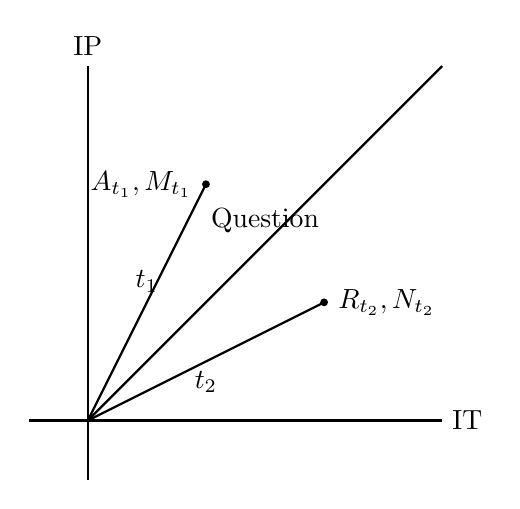
\begin{tikzpicture}[scale=1.5, axis/.style={thick}, vector/.style={thick},
                    point/.style={circle, inner sep=1pt, fill, color=black}
]

% Coordinate axes
\draw[axis] (-0.5, 0) -- (3, 0) node[right] {IT};
\draw[axis] (0, -0.5) -- (0, 3) node[above] {IP};

% Points for t1 and t2
\coordinate (t1) at (1, 2);
\coordinate (t2) at (2, 1);
\coordinate (iq) at (3, 3);

% Vectors for t1, t2, and the sum
\draw[vector] (0, 0) -- node[pos=0.5, above] {$t_1$} (t1);
\draw[vector] (0, 0) -- node[pos=0.5, below] {$t_2$} (t2);
\draw[vector] (0, 0) -- node[pos=0.5, above] {Question} (iq);

% Points and labels for t1 and t2
\node[point, label={left:$A_{t_1}, M_{t_1}$}] at (t1) {};
\node[point, label={right:$R_{t_2}, N_{t_2}$}] at (t2) {};

\end{tikzpicture}
\caption{\label{fig:InterestingQuestion}Example of an interesting quetion.}
\end{figure}

In practice, we must calculate all possible combinations of topics with high interestingness as tools and those with high interestingness as problems. We then select the combinations with the highest interestingness as questions. Naturally, most questions generated using this approach will be meaningless, much like those arising during brainstorming sessions when researchers attempt to identify new tools for tackling difficult problems.

This methodology can be applied in other scenarios as well. For instance, a researcher familiar with problem $p$ might be interested in finding applicable tools to solve it. Similarly, a researcher specializing in tool $t$ may be interested in discovering open problems where his expertise can be applied.

The above procedure can be easily generalized to encompass multiple tools and possibly multiple problems. This leads to the application of two tools to a given problem ($ t_1 + t_2 \rightarrow p$), the application of a single tool to the combination of two problems ($t \rightarrow p_1 + p_2$), and so on. The exact meaning of these tool and problem combinations depends on the topics themselves.

An interesting question is intradisciplinary if it combines two topics that are studied in the framework of the same research area (e.g., computer science). An interesting question is interdisciplinary if it combines two topics of different research areas (e.g., computer science and philosophy). In principle, the most innovative questions would be interdisciplinary questions, because the probability that somebody has thought about them is lower, since it requires specialists in both research areas working together to come up with that particular question.

\begin{definition}\index{Intradisciplinary question}\index{Interdisciplinary question}
Let $\mathcal{A}\subseteq\mathcal{T}$ be a research area. The question $Q_{t\to p}$ is \emph{intradisciplinary}\index{Intradisciplinary question} if $t,p\in\mathcal{A}$; otherwise it is \emph{interdisciplinary}\index{Interdisciplinary question}.
\end{definition}

\begin{example}
We could combine the topics with high interestingness as tools found in the area of "computer science" with those topics with high interestingness as problems found in the area of "biochemistry" in order to find new interesting interdisciplinary questions. Some examples of the kind of questions we can find with this approach include: "can we use regular expressions to identify DNA genes?" or "can we use a recursive algorithm to characterize proteins tertiary structure?"
\end{example}

The most innovative questions tend to be interdisciplinary, as they have a lower likelihood of having been considered previously. This is because they require collaboration between specialists from different research areas. 

%
% Section: New Research Topics
%
\section{New Topics}
\label{sec:new-topics}

The area composed by the unknown unknown problems is a highly interesting one, since it contains those research topics that will be addressed in the future. One of the main goals of this book is to help scientists discover the topics that lay in this unknown unknown area, since that would bring to the present the research problems of the future. In this section we focus on how to indentify the topics hidden in the unknown unknown area.

\begin{definition}\index{New topic}
Given $t_1,t_2\in T'$, a (candidate) \emph{new topic} from their combination is the unordered pair
\[
S_{\{t_1,t_2\}}=\{t_1,t_2\}.
\]
Associate $v(t)=(\tilde{N}(t),\bar{R}(t))$ and define the combination vector $v^\oplus(t_1,t_2)=v(t_1)+v(t_2)$.
\end{definition}

The exact meaning of the new topic that results as the combination of topics $t_{1}$ and $t_{2}$ is left to the creative interpretation of the researcher.

\begin{definition}\index{Interestingness of a new topic}
We define the interestingness of $S_{\{t_1,t_2\}}$ as
\[
IS(\{t_1,t_2\})=\frac{\sqrt{\,IT(t_1)^2+IT(t_2)^2\,}}{\sqrt{2}}
\]

\end{definition}

In practice, what we have to do is to compute all possible combination of those topics with very large interestingness as problems $IP_{t}$ with themselves, and select the combinations with higher $IS$. Of course, some of the combinations generated would be totally meaningless. Advanced techniques from the area of natural language processing or machine learning could be used to try filter out those nonsense combinations.

\begin{definition}\index{Intradisciplinary new topic}\index{Interdisciplinary new topic}
Let $\mathcal{A}\subseteq\mathcal{T}$. The new topic $S_{\{t_1,t_2\}}$ is \emph{intradisciplinary} if $t_1,t_2\in\mathcal{A}$; otherwise it is \emph{interdisciplinary}.
\end{definition}

Again, the most innovative new topics would be by the combination of interdisciplinary topics, because the probability that somebody has already though about them is lower.

%
% References
%

\section*{References}

The following works provide theoretical and philosophical foundations for the concepts of interestingness, maturity, and the combination of topics as tools and problems.

\cite{chalmers2013thing} An accessible introduction to the philosophy of science, addressing how scientific questions are formulated, evaluated, and justified.

\cite{pearl2019book} Introduces the principles of causal reasoning, crucial for determining whether applying one topic as a tool can effectively address another as a problem.

\cite{popper2014conjectures} Discusses falsifiability, novelty, and the importance of bold conjectures—foundational ideas for the “new and original” criterion.

\cite{shmueli2010explain} Clarifies the distinction between explanatory and predictive goals, helping to differentiate between topics valuable as problems versus tools.

\cite{van1980scientific} Explores the aims of science, model construction, and empirical adequacy, offering a philosophical context for defining “interesting” research.
